\documentclass[tikz,convert={density=150,size=600,outext=.png}]{standalone}
\usetikzlibrary{shapes, calc, arrows, fit, positioning, decorations, patterns,
  decorations.pathreplacing, chains, snakes}

\begin{document}
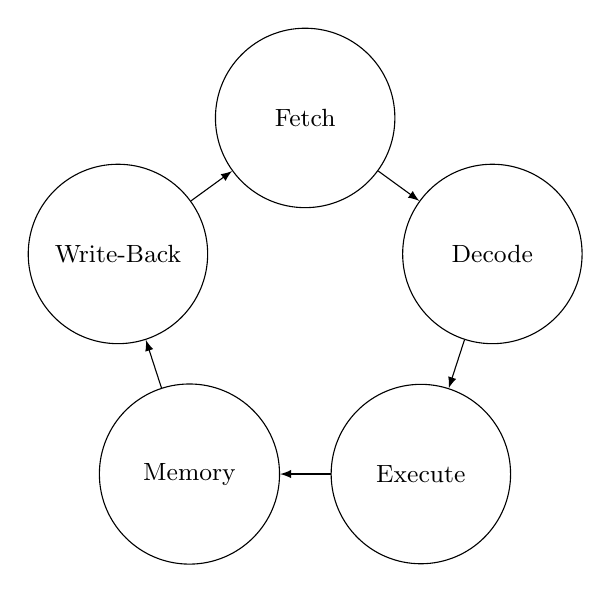
\begin{tikzpicture}[font=\footnotesize, >=latex]
  \foreach \A/\T in {  90/{Fetch},
                       18/{Decode},
                      306/{Execute},
                      234/{Memory},
                      162/{Write-Back}
  } {
  \node[draw, circle, text width = 2cm, text centered](stage\A) at (\A:2.5cm) {\small\T};
  }

  \draw[->, ] (stage90) -- (stage18);
  \draw[->, ] (stage18) -- (stage306);
  \draw[->, ] (stage306) -- (stage234);
  \draw[->, ] (stage234) -- (stage162);
  \draw[->, ] (stage162) -- (stage90);
\end{tikzpicture}
\end{document}
